\documentclass[uplatex,12pt]{jsarticle}
\usepackage[dvipdfmx]{graphicx}
\usepackage{url}
\usepackage{listings,jlisting}
\usepackage{ascmac}
\usepackage{amsmath,amssymb}

%ここからソースコードの表示に関する設定
\lstset{
  basicstyle={\ttfamily},
  identifierstyle={\small},
  commentstyle={\smallitshape},
  keywordstyle={\small\bfseries},
  ndkeywordstyle={\small},
  stringstyle={\small\ttfamily},
  frame={tb},
  breaklines=true,
  columns=[l]{fullflexible},
  numbers=left,
  xrightmargin=0zw,
  xleftmargin=3zw,
  numberstyle={\scriptsize},
  stepnumber=1,
  numbersep=1zw,
  lineskip=-0.5ex
}
%ここまでソースコードの表示に関する設定

\title{知能プログラミング演習II 課題3}
\author{グループ8\\
  29114116 増田大輝\\
}
\date{2019年10月25日}

\begin{document}
\maketitle

\paragraph{提出物} rep3
\paragraph{グループ} グループ8

\paragraph{メンバー}
\begin{tabular}{|c|c|c|}
  \hline
  学生番号&氏名&貢献度比率\\
  \hline\hline
  29114003&青山周平&NoData\\
  \hline
  29114060&後藤拓也&NoData\\
  \hline
  29114116&増田大輝&NoData\\
  \hline
  29114142&湯浅範子&NoData\\
  \hline
  29119016&小中祐希&NoData\\
  \hline
\end{tabular}



\section{課題の説明}
\begin{description}
\item[課題3-1] セマンティックネットのプログラムを参考に,グループメンバー全員(およびその周辺人物)についてのセマンティックネットを構築せよ.\\
・個人レポートには自分のみ(とその周辺)に関するセマンティックネットを示し,グループレポートには全員(とその周辺)に関するセマンティックネットを示せ.
\item[課題3-2] フレームのプログラムを参考に,自分達の興味分野に関する知識をフレームで表現せよ.その分野の知識を表す上で必須となるスロットが何かを考え,クラスフレームを設計すること. \\
・個人レポートには自分が作ったインスタンスフレームのみ(クラスフレームの設計担当者はクラスフレームも)を示し,グループレポートにはクラスフレームおよび全員分のインスタンスフレームを示せ.
\item[課題3-3] 課題3-1または3-2で作った知識表現を用いた質問応答システムを作成せよ.
なお,ユーザの質問は英語や日本語のような自然言語が望ましいが,難しければ課題2で扱ったような変数を含むパターン (クエリー) でも構わない.
\end{description}

\section{課題3-1}
\begin{screen}
    セマンティックネットのプログラムを参考に,グループメンバー全員(およびその周辺人物)についてのセマンティックネットを構築せよ.\\
    ・個人レポートには自分のみ(とその周辺)に関するセマンティックネットを示し,グループレポートには全員(とその周辺)に関するセマンティックネットを示せ.
\end{screen}

\subsection{手法}
教科書3.1節のセマンティックネットのプログラムを参考にしてテキストファイルからデータを読み込み,セマンティックネットを構築する.
semantic\_net/下に以下のプログラムを配置した.
\begin{description}
    \item[Node.java] セマンティックネットを構成するノード.主に名詞に当たる.
    \item[Link.java] ノード間を結ぶリンク.主に動詞に当たる.
    \item[SemanticNet.java] ノードとリンクにより構成されるセマンティックネット.
    \item[SemanticNetTest.java] テキストファイルのデータからセマンティックネットを構成する.
\end{description}
特に,SemanticNetTest.javaでは,指定したテキストファイルから各学生のデータを読むことにより,名詞をノード,動詞をリンクとしてセマンティックネットを構築する.
以下に,今回の課題で作成した個人のセマンティックネットを示す.
\begin{figure}[!hbt]
    \centering
    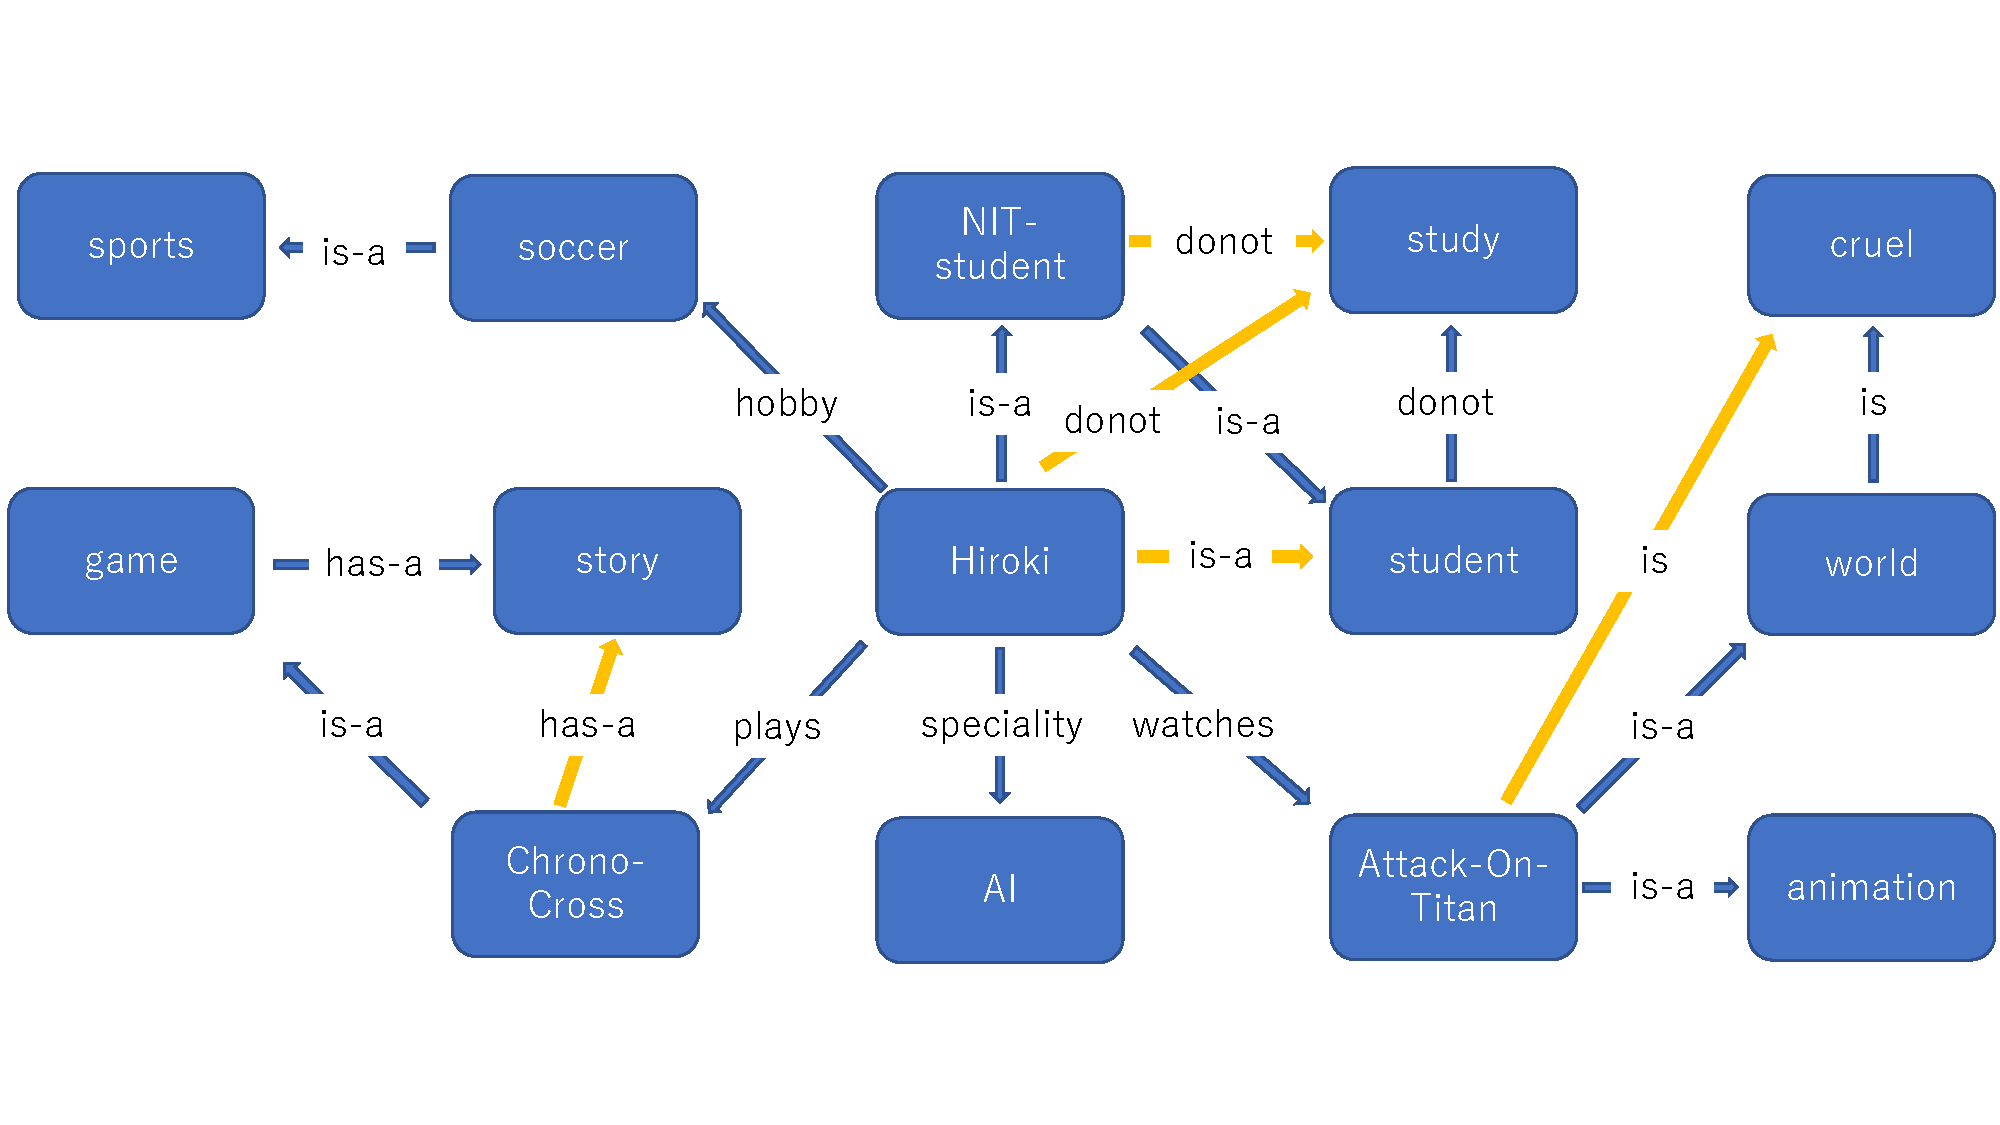
\includegraphics[scale=0.40]{images/masuda_semantic_net.pdf}
    \caption{増田セマンティックネットの概念図}
\end{figure}

\newpage

\subsection{実装}
この課題では,教科書のセマンティックネットのプログラムを利用するSemanticNetTest.javaを作成した.
このクラスでは,実行時に第一引数として渡された文字列に該当するmembers/下とqueries/下のテキストファイルからデータを読み取って実行する. \\
以下で,作成したメソッドとその役割について簡単に述べる.
\begin{description}
    \item[readTextFile] テキストファイルファイルからデータを読み込み,List<String>として返却する.
    \item[splitStatement] 単文を空白で分割する.
    \item[addLink] 分割された単文からリンクを作成し,セマンティックネットに追加する.
    \item[addQuery] 分割された単文からクエリを作成し,セマンティックネットに追加する.
\end{description}
以上の関数を組み合わせ,テキストファイルから読み込まれたデータからセマンティックネットを構築・検索し,出力を行うようにmain()文に実装した.
main文内における具体的な実装手順を以下のソースコードに示す.
\begin{lstlisting}[caption=SemanticNetTest.javaのmain()内部, label=mid]
    SemanticNet sn = new SemanticNet();
    if(args.length == 1) {
        // 個人のデータをmembers/下のテキストファイルから読み込む
        List<String> statementList = readTextFile("members/"+args[0]+".txt");
        for(String statement: statementList) {
            // 単文を主格・動詞・目的格に3分割する
            List<String> splitList = splitStatement(statement);
            // セマンティックネットにリンクを追加する
            addLink(sn, splitList);
        }
        sn.printLinks();
        sn.printNodes();
        
        // 検索クエリをqueries/下のテキストファイルから読み込む
        List<String> queryList = readTextFile("queries/"+args[0]+".txt");
        ArrayList<Link> query = new ArrayList<Link>();
        for(String queryStatement: queryList) {
            // 単文を主格・動詞・目的格に3分割する
            List<String> splitList = splitStatement(queryStatement);
            // 新たなクエリを追加する
            addQuery(query, splitList);
        }
        sn.query(query);
    }
\end{lstlisting}
このソースコードからも読み取れるように,セマンティックネットを構築する際のプログラム(3〜10行目)と,
クエリを追加する際のプログラム(14〜22)では,構造が非常に似ている. \\
これは,readTextFileメソッドとsplitStatementメソッドによって両者で共通する処理が行われるためである. \\
反対に,両者の差をそれぞれaddLinkメソッドとaddQueryメソッドによって吸収している. \\
共通する処理をメソッドに切り出すことでmain()文内の複雑化を防ぐと共に,各種メソッドを目的が明確かつ汎用性があるように設計した.
このため,main()文では目的に応じて使用するメソッドを切り替えているに止まり,差分の吸収機能を果たすのみであることから構造が単純なものとなっている.

\subsection{実行例}
セマンティックネットを構築するためのデータとして以下のようなデータをsemantic\_net/members/下に用意した.
\begin{lstlisting}[caption=semantic\_net/members/masuda.txt, label=mid]
    soccer is-a sports
    Hiroki is-a NIT-student
    Hiroki speciality AI
    Chrono-Cross is-a game
    game has-a story
    Hiroki hobby soccer
    Hiroki plays Chrono-Cross
    NIT-student is-a student
    student donot study
    Attack-On-Titan is-a animation
    Hiroki watches Attack-On-Titan
    Attack-On-Titan is-a world
    world is cruel
\end{lstlisting}
また,クエリによる検索を行うための以下のデータをsemantic\_net/queries/下に用意した.
\begin{lstlisting}[caption=semantic\_net/queries/masuda.txt, label=mid]
    ?y plays Chrono-Cross
    ?y is-a student
    ?y hobby soccer
    ?y watches Attack-On-Titan
\end{lstlisting}
semantic\_net/下においてコンパイル後に以下のコマンドを実行することで対象のテキストファイルに含まれるデータのセマンティックネットを構築できる. \\
java SemanticNetTest [名前] \\
次に,"java SemanticNetTest masuda"の実行例を示す.
\begin{lstlisting}[caption=java SemanticNetTest masudaの実行例, label=mid]
    ~/Programming2/Work3/semantic_net
    ●java SemanticNetTest masuda                                                                                                                                                                                           【 fix/semantic_net 】
    *** Links ***
    soccer  =is-a=>  sports
    Hiroki  =is-a=>  NIT-student
    Hiroki  =speciality=>  AI
    Chrono-Cross  =is-a=>  game
    game  =has-a=>  story
    ( Chrono-Cross  =has-a=>  story )
    Hiroki  =hobby=>  soccer
    Hiroki  =plays=>  Chrono-Cross
    NIT-student  =is-a=>  student
    ( Hiroki  =is-a=>  student )
    student  =donot=>  study
    ( NIT-student  =donot=>  study )
    ( Hiroki  =donot=>  study )
    Attack-On-Titan  =is-a=>  animation
    Hiroki  =watches=>  Attack-On-Titan
    Attack-On-Titan  =is-a=>  world
    world  =is=>  cruel
    ( Attack-On-Titan  =is=>  cruel )
    *** Nodes ***
    soccer
    sports
    Hiroki
    NIT-student
    AI
    Chrono-Cross
    game
    story
    student
    study
    Attack-On-Titan
    animation
    world
    cruel
    *** Query ***
    ?y  =plays=>  Chrono-Cross
    ?y  =is-a=>  student
    ?y  =hobby=>  soccer
    ?y  =watches=>  Attack-On-Titan
    [{?y=Hiroki}]
\end{lstlisting}

\subsection{考察}
セマンティックネットを構築する際に特に注目したのが,is-a関係による特性の継承である.
\verb|Chrono-Cross  =is-a=>  game| によって下位概念である「Chrono-Cross」から上位概念である「game」が関連付けられ,
\verb|game  =has-a=>  story| によって「game」に特性が紐づけられる.
結果として, \verb|Chrono-Cross  =has-a=>  story| が導出される実装から,知識表現とオブジェクト指向プログラミングの親和性の良さを体感した. \\
セマンティックネットを活用することによって,単純なデータの列挙から新たな知識を導出できることができる. \\
しかし,知識推論は一般から具体への方向にのみ働くことに注意が必要である.


\section{課題3-2}
\begin{screen}
    フレームのプログラムを参考に,自分達の興味分野に関する知識をフレームで表現せよ.その分野の知識を表す上で必須となるスロットが何かを考え,クラスフレームを設計すること. \\
    ・個人レポートには自分が作ったインスタンスフレームのみ(クラスフレームの設計担当者はクラスフレームも)を示し,グループレポートにはクラスフレームおよび全員分のインスタンスフレームを示せ.
\end{screen}
クラスフレーム設計担当者であるので,3.1節にて設計したクラスフレームを示す.

\subsection{手法}
教科書3.1節のフレームのプログラムを参考にしてテキストファイルからデータを読み込み,フレームを構築する.
semantic\_net/下に以下のプログラムを配置した.
\begin{description}
    \item[AIFrame.java] フレームのスーパークラス.
    \item[AIClassFrame.java] フレームの具体化クラス.クラスフレームを表す. 
    \item[AIInstanceFrame.java] フレームの具体化クラス.インスタンスフレームを表し,いずれかのクラスフレームのインスタンスである. 
    \item[AISlot.java] フレームが持つスロット. 
    \item[AIDemonProc.java] デモン手続きのスーパークラス.
    \item[AIDemonProcReadTest.java] デモン手続きの具体化クラス.読み込みデモン手続きを行う.
    \item[AIDemonProcWriteTest.java] デモン手続きの具体化クラス.書き込みデモン手続きを行う.
    \item[AIWhenConstructedProc.java] クラスをデモン手続きとして利用するための抽象クラス. 
    \item[AIFrameSystem.java] フレームシステムを表す.
    \item[FrameTest.java] テキストファイルのデータからフレームを構成する.  
\end{description}
特に,FrameTest.javaでは,ゲームソフトを表すクラスフレームを作成し,対応デバイス・本体価格・課金額・累計金額の四種類のスロットを作成する.
その後,インスタンスフレームを作成し,グループメンバーそれぞれが提案したゲームソフトのフレームとする. \\
以下に,ゲームクラスフレームのスロットについて示す.
\begin{description}
    \item[device] 対応ソフト,すなわち,ゲームソフトのプラットフォームを指定する.String型オブジェクトとし,"device"をデフォルトとする.
    \item[value] 本体価格を指定する.Integer型のオブジェクトとし,0をデフォルトとする.
    \item[charges] 課金額を指定する.Integer型のオブジェクトとし,0をデフォルトとする.
    \item[tribute] 累計金額を指定する.Integer型のオブジェクトとし,value+chargesをデフォルトとする.
\end{description}
累計金額を計算するにあたって,デモン手続きを用いて本体価格と課金額の和をとる.
スロット値を読み取る際に計算を行うので,AIDemonProcReadTest.javaクラスに記述を追加した. \\
次に,クラスフレームの図を示す.
\newpage
\begin{figure}[!hbt]
    \centering
    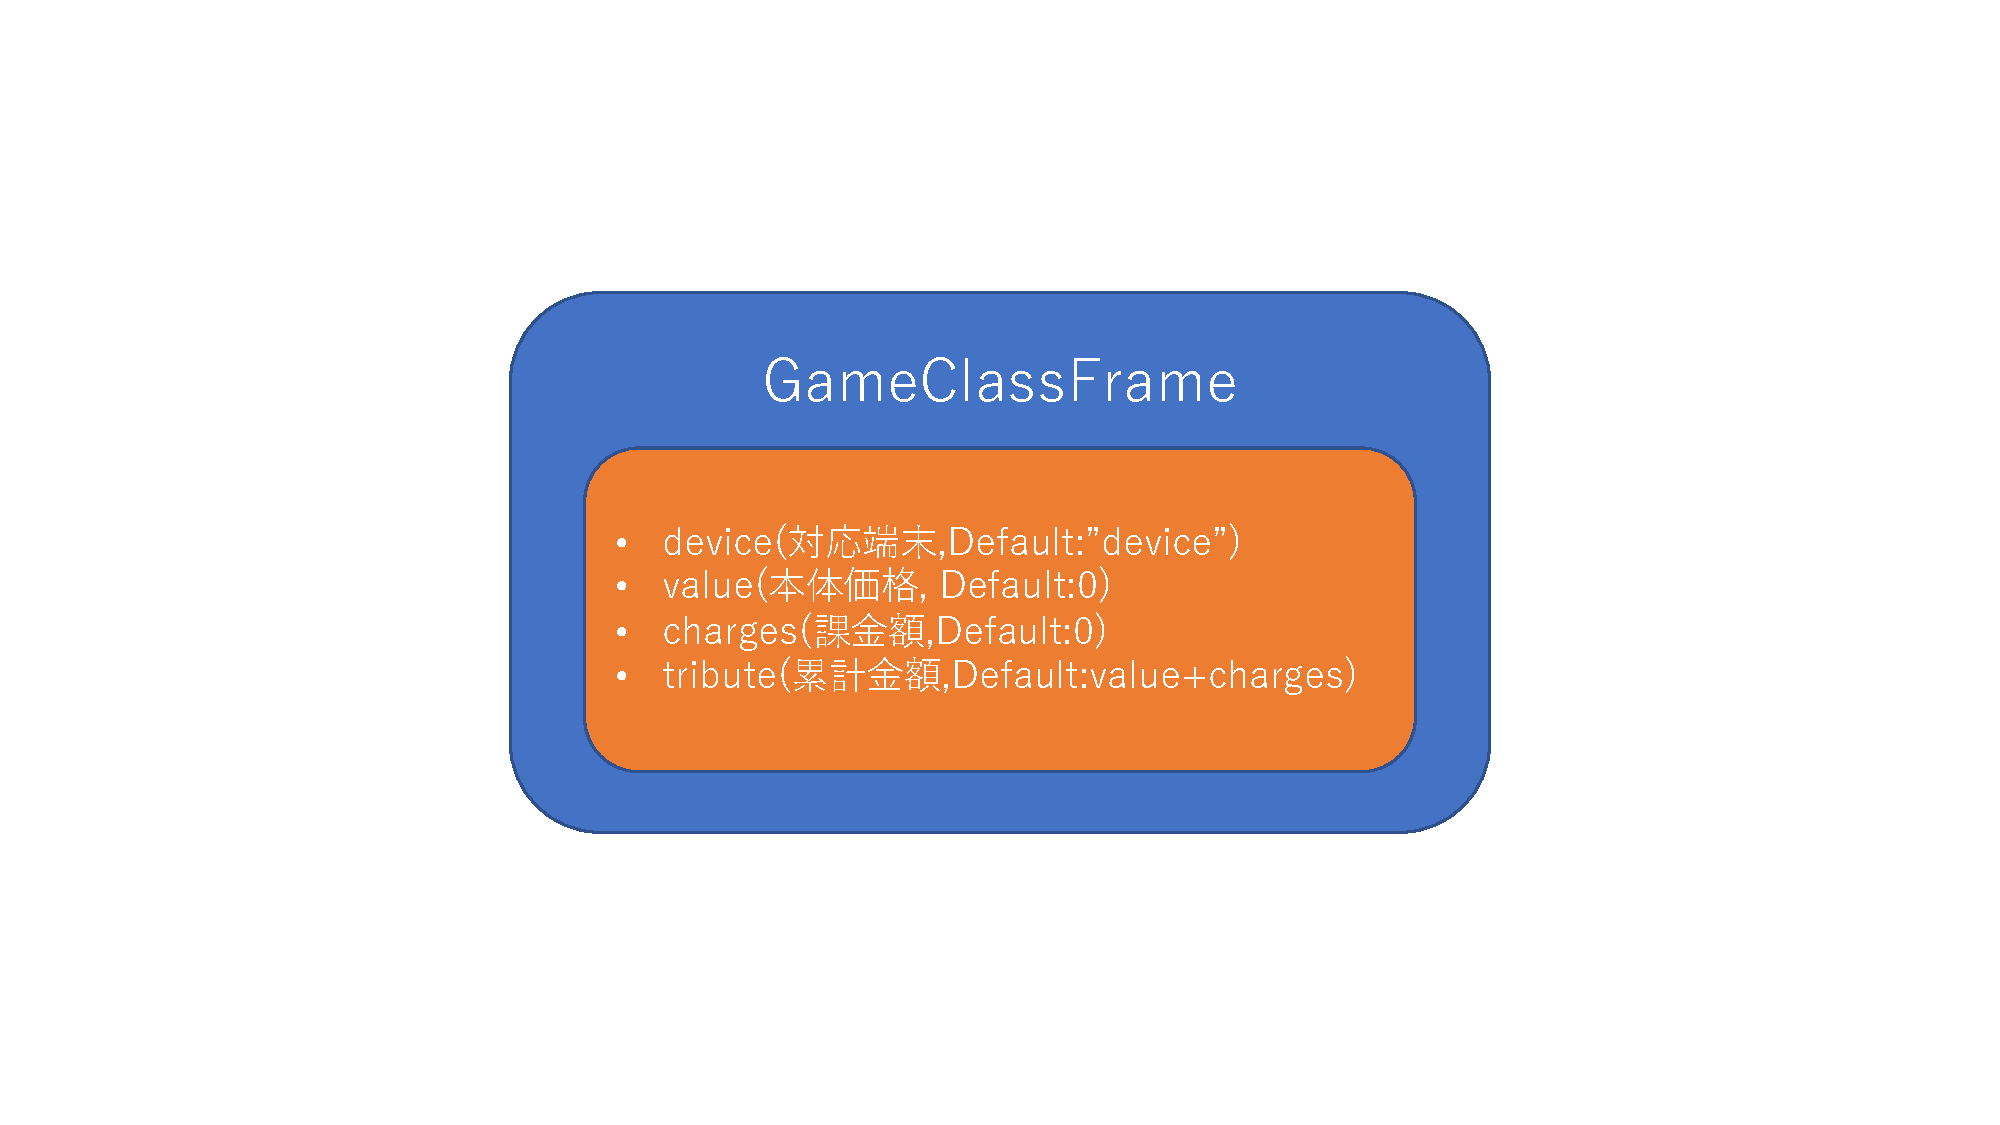
\includegraphics[scale=0.35]{images/game_class_frame.pdf}
    \caption{ゲームクラスフレームの概念図}
\end{figure}

以下に,私個人が作成したインスタンスフレームMonster-Hunterフレームの図を示す. \\
ただし,各スロット名の横の値は,書き込みデモン手続きによって更新されるインスタンスフレームの各スロットの値である.
\begin{figure}[!hbt]
    \centering
    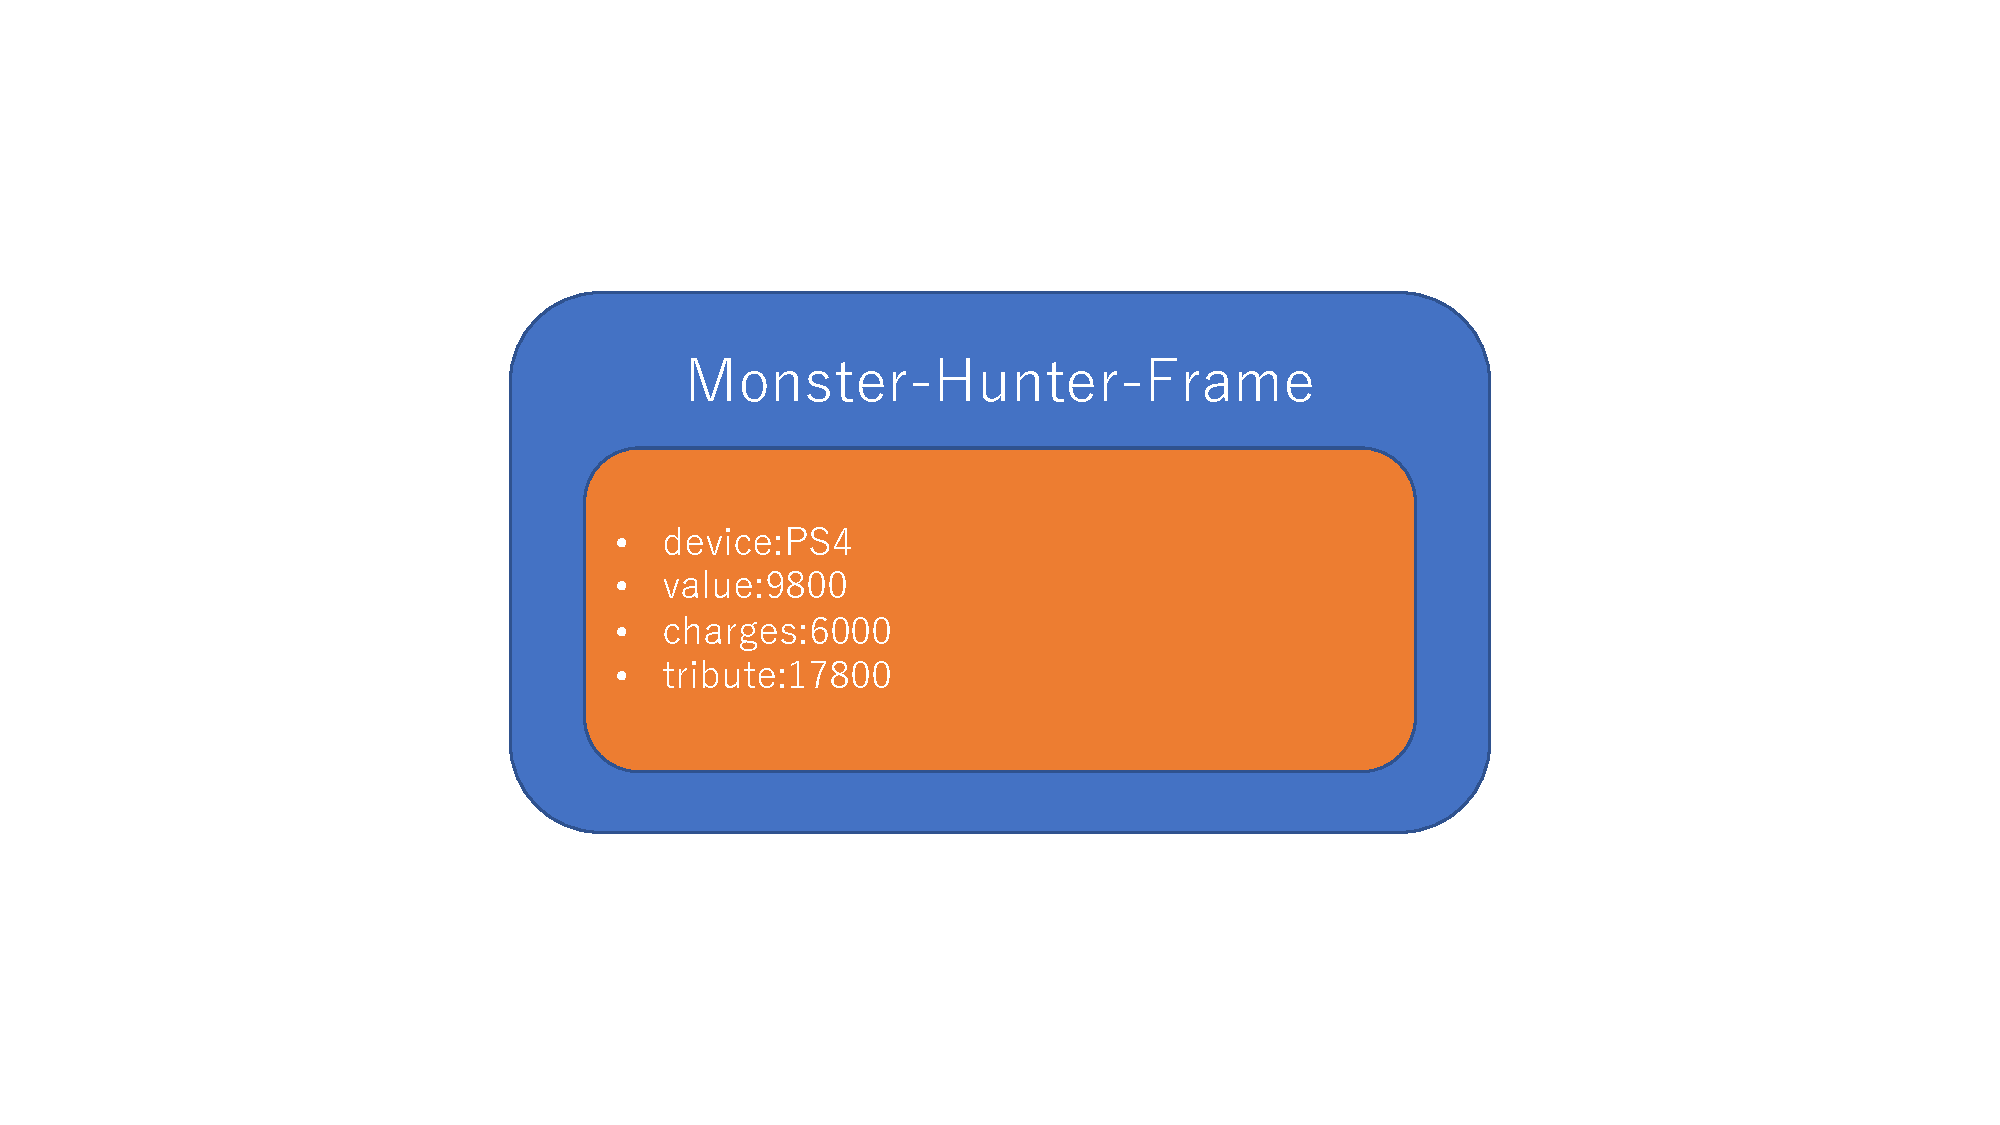
\includegraphics[scale=0.35]{images/monster_hunter_frame.pdf}
    \caption{Monster-Hunterフレームの概念図}
\end{figure}

\subsection{実装}
この課題では,教科書のフレームのプログラムを利用するFrameTest.javaを作成した.
このクラスでは,実行時に第一引数として渡された文字列に該当するgames/下のテキストファイルからデータを読み取って実行する. \\
以下で,作成したメソッドとその役割について簡単に述べる.
\begin{description}
    \item[readTextFile] テキストファイルファイルからデータを読み込み,List<String>として返却する.
    \item[defineClassFrame] クラスフレームとスロットを定義.また,デモン手続きを設定する.
    \item[outputSlots] スロット値の一覧を表示する.
\end{description}
また,インスタンスフレームのスロット値の更新と出力は以下のソースコードにある順で行う.
\begin{lstlisting}[caption=インスタンスフレームのスロット値の更新と出力プログラム, label=mid]
    // device,value,charges,tribute はデフォルト値
    System.out.println( "device,value,charges,tribute はデフォルト値" );
    outputSlots(fs, instanceName, false);
    System.out.println();

    // tribute はデフォルト値
    System.out.println( "tribute はデフォルト値" );
    fs.writeSlotValue( instanceName, "device", new String(slotList.get(0)));
    fs.writeSlotValue( instanceName, "value", new Integer(slotList.get(1)) );
    fs.writeSlotValue( instanceName, "charges", new Integer(slotList.get(2)) );
    outputSlots(fs, instanceName, false);
    System.out.println();

    // 再びデフォルト値
    System.out.println( "再びデフォルト値" );
    fs.writeSlotValue( instanceName, "tribute", new Integer(slotList.get(3)) );
    outputSlots(fs, instanceName, true);
\end{lstlisting}
さらに,以下の読み込みデモン手続きを用いて,$tribute = value + charges$を実装する.
\begin{lstlisting}[caption=AIDemonProcReadTest.javaにおける読み込みデモン手続き, label=mid]
    Object value = inFrame.readSlotValue( inFrameSystem, "value", false );
    Object charges = inFrame.readSlotValue( inFrameSystem, "charges", false );
    if ( value instanceof Integer && charges instanceof Integer) {
        int v = ((Integer) value).intValue();
        int c = ((Integer) charges).intValue();
        return AIFrame.makeEnum( new Integer( (int) v + c) );
    }
\end{lstlisting}

\subsection{実行例}
フレームを構築するためのデータとして,以下のデータをframe/games/下に用意した.
\begin{lstlisting}[caption=frame/games/Monster-Hunter.txt, label=mid]
    PS4
    9800
    6000
    17800
\end{lstlisting}
frame/下においてコンパイル後に以下のコマンドを実行することで対象のテキストファイルに含まれるデータのフレームを構築できる. \\
java FrameTest [ゲーム名] \\
次に,"java FrameTest Monster-Hunter"の実行例を示す.
\begin{lstlisting}[caption=java FrameTest Monster-Hunterの実行例, label=mid]
    ~/Programming2/Work3/frame
    ●java FrameTest Monster-Hunter                                                                                                                                                                                                【 fix/frame 】
    クラスフレーム:game

    インスタンスフレーム:Monster-Hunter

    device,value,charges,tribute はデフォルト値
    スロット値一覧
    device:device
    value:0
    charges:0
    tribute:0

    tribute はデフォルト値
    スロット値一覧
    device:PS4
    value:9800
    charges:6000
    tribute:15800

    再びデフォルト値
    スロット値一覧
    device:device
    value:0
    charges:0
    tribute:15800
\end{lstlisting}

\subsection{考察}
フレームは概念的にはセマンティックネットを拡張したものであり,クラスフレームからの継承の要素を残しつつも,
それぞれのフレームが直接スロットを保持することによって,特性の記述も可能である.
また,セマンティックネットとの大きな違いとして上げられる点として,デモン手続きが存在することによって,
クラスフレームのスロットデータをデフォルト値として保持しながらも,インスタンスフレームでスロットデータの書き換えが可能である.
また,データ格納の性質上,セマンティックネットは自然言語からの構築に適していると考えられるが,
フレームの場合はデータベースからの構築に適していると考えられる.
それぞれの概念の得意なデータの形式を考えることで,より効果的な知識システムを構築できると考えられる.

% 参考文献
\begin{thebibliography}{99}
\bibitem{notty} Javaによる知能プログラミング入門 --著:新谷 虎松 \\
\end{thebibliography}

\end{document}